\documentclass{article}
\usepackage{indentfirst,latexsym,bm}
\usepackage{graphics}
\usepackage{color}
%\usepackage{CJK}
\usepackage{amsmath}
\usepackage{amssymb}
\usepackage{dsfont}
\usepackage{mathrsfs} %For \mathscr
\usepackage[latin1]{inputenc}
\usepackage{tikz}
\usetikzlibrary{trees}
\usepackage{listings}
\usepackage{csquotes}
\usepackage[top=0.8in, bottom=.8in, left=0.5in, right=0.5in]{geometry}
\usepackage{hyperref}
\setlength{\parindent}{1em}

\def\dsst{\displaystyle}
\pagenumbering{arabic}
\begin{document}
%\pagestyle{empty}
\title{Week 3 Lecture Video Explanations Part II}
\author{Duke University}
\date{}
\maketitle 

\section{Paradoxes and Choosing Priors}

In this video, we calculate the Bayes factor of the Extra-Sensory Perception (ESP) example to illustrate the situation how paradoxes appear. In this example, we have sample size $n = 104,490,000$ with the number of ``success" (the number of 1's generated by machine) being 52,263,471. This is a Binomial process. Our goal is to compare the proportion of 1's with the usual true proportion 0.5. We might adopt the method we used in the \textbf{Comparing Two Proportions} section to calculate the Bayes factor. However, since the sample size is huge, we may also assume the proportion follows the Normal distribution with known variance, to reduce our calculation. 

\subsection{Review: Frequentist Approach}

Here we use $\bar{Y} = \dsst \frac{52,263,471}{104,490,000} \approx 0.5001768$ to denote the proportion of 1's generated by the machine under the ESP assumption. Notice that this proportion is also the mean of all the numbers generated by the machine. That is why in the video we use the mean notation to denote the proportion. \\

We have 2 hypotheses. Since we will compare this approach with the Bayesian approach later on, we will not use $H_0$ and $H_a$ to distinguish the null hypothesis and alternative hypothesis, instead, we set:
\begin{align*}
H_1: & \bar{Y} = 0.5\\
H_2: & \bar{Y} \neq 0.5
\end{align*}

Since the number of successes and the number of failures are both larger than 5, we can assume the sample satisfies the assumption of a $z$-test to test the proportion. Under the frequentist approach, we calculate the $z$-score, 
$$ z^* = \frac{\bar{Y} - 0.5}{\sqrt{(0.5)(1 - 0.5) / n}} = \frac{0.5001768 - 0.5}{\sqrt{0.25 / 104,490,000}} \approx 3.61396 $$

The two-sided $p$-value is 0.000302. Under the significant level $\alpha = 0.05$, we will reject the null hypothesis that $\bar{Y} = 0.5$. 

\subsection{Bayesian Approach}

To compare, we calculate the Bayes factor $\text{BF}[H_1:H_2]$, and derive the posterior probability of $H_1$ under the observed data. We would like to see whether the Bayes factor provide strong evidence that supports $H_1$ (or $H_2$). \\

As we have stated, due to the large sample size, by the Central Limit Theorem, we can assume the proportion $\bar{Y}$ is normally distributed with known variance $\sigma^2/n$, where $\sigma^2$ is the variance of the data(right??? or just variance under true proportion???)\\

Under $H_1$, we assume $\bar{Y} = 0.5$. So the distribution of $\bar{Y}$ under $H_1$ is $\bar{y}~|~H_1 \sim \mathcal{N}(0.5, \sigma^2 / n),$ 
$$\ f(\bar{y}~|~H_1) = \dsst \frac{1}{\sqrt{2\pi\sigma^2/n}}\exp\left(-\frac{(\bar{y}-0.5)^2}{\sigma^2/n}\right).$$ \\

Under $H_2$, we do not know the specific mean of $\bar{Y}$, $\mu$. Therefore, we need to set up a prior of $\mu$, and update this prior after observing the data from the study. Here we will use the Normal-Normal conjugate family since we assume the variance of $\bar{Y}$ is known. We set the prior distribution of $\mu$ under $H_2$ to be
$$ \mu~|~H_2 \sim \mathcal{N}(0.5, \frac{\sigma^2}{n_0}), \qquad \pi(\mu~|~H_2) = \frac{1}{\sqrt{2\pi\sigma^2/n_0}}\exp\left(-\frac{(\mu - 0.5)^2}{2\sigma^2/n_0}\right). $$
(We use $\dsst \frac{\sigma^2}{n_0}$ instead of $\tau^2$ for calculation convenience. Recall that changing $n_0$ can change the precision of the distribution.)\\

By the Normal-Normal conjugacy, we can show that under $H_2$
$$ \pi^*(\mu~|~\bar{y}, H_2) = \frac{f(\bar{y}~|~\mu, H_2)\pi(\mu~|~H_2)}{\dsst \int f(\bar{y}~|~\mu, H_2)\pi(\mu~|~H_2)\, d\mu},\qquad \mu~|~\bar{y}, H_2 \sim \mathcal{N}(\nu^*, (\tau^*)^2), $$
where
$$ \nu^* = \frac{\nu \frac{\sigma^2}{n} + \bar{y}\frac{\sigma^2}{n_0}}{\frac{\sigma^2}{n} + \frac{\sigma^2}{n_0}} = \frac{0.5n_0 + \bar{y}n}{n + n_0}, $$
$$ (\tau^*)^2 = \frac{\frac{\sigma^2}{n}\frac{\sigma^2}{n_0}}{\frac{\sigma^2}{n}+\frac{\sigma^2}{n_0}} = \frac{\sigma^2}{n+n_0}. $$

Hence,
$$ \mu~|~\bar{y}, H_2\sim \mathcal{N}\left(\frac{0.5n_0+\bar{y}n}{n+n_0},\ \frac{\sigma^2}{n+n_0}\right) \qquad \pi^*(\mu~|~\bar{y}, H_2) = \frac{1}{\sqrt{2\pi \sigma^2/(n+n_0)}}\exp\left(-\frac{\left(\mu - \frac{0.5n_0+\bar{y}n}{n+n_0}\right)^2}{2\sigma^2/(n+n_0)}\right). $$
(You may notice that we have added $H_1$ and $H_2$ into the conditional probability distributions. We use these notations to distinguish the situation under each hypothesis. But the formula to calculate the posterior distribution is still the same.)

\subsubsection*{Calculate the Bayes Factor and the Posterior Probability of $H_1$}

Bayes factor in the continuous case is the ratio between the (marginal) probability distributions of $\bar{Y}$ under two hypotheses
$$ \text{BF}[H_1:H_2] = \frac{f(\bar{y}~|~H_1)}{ \dsst \int f(\bar{y}~|~\mu, H_2)\pi(\mu~|~H_2)\, d\mu}. $$

We already have
$$ \bar{y}~|~H_1\ \sim  \mathcal{N}(0.5, \frac{\sigma^2}{n}), \qquad f(\bar{y}~|~H_1) = \frac{1}{\sqrt{2\pi\sigma^2/n}}\exp\left(-\frac{(\bar{y}-0.5)^2}{2\sigma^2/n}\right). $$

To calculate the denominator, we use the formula by which we obtained the posterior distribution of $\mu$ under $H_2$, similar to what we did in the \textbf{Comparing Two Proportions Using Bayes Factors} session
\begin{align*}
\int f(\bar{y}~|~\mu, H_2)\pi(\mu~|~H_2)\, d\mu = & \frac{f(\bar{y}~|~\mu, H_2)\pi(\mu~|~H_2)}{\pi^*(\mu~|~\bar{y}, H_2)} \\
= & \left[\frac{1}{\sqrt{2\pi\sigma^2/n}}\exp\left(-\frac{(\bar{y}-\mu)^2}{2\sigma^2/n}\right)\right]\times \left[\frac{1}{\sqrt{2\pi\sigma^2/n_0}}\exp\left(-\frac{(\mu - 0.5)^2}{2\sigma^2/n_0}\right)\right] \\
& \div \left[\frac{1}{\sqrt{2\pi\sigma^2/(n+n_0)}}\exp\left(-\frac{\left(\mu-\frac{0.5n_0+\bar{y}n}{n+n_0}\right)^2}{2\sigma^2/(n+n_0)}\right)\right] \\ 
= & \frac{1}{\sqrt{2\pi\sigma^2(n+n_0)/(n\cdot n_0)}}\exp\left(-\frac{(\bar{y}-\mu)^2}{2\sigma^2/n}-\frac{(\mu-0.5)^2}{2\sigma^2/n_0}+\frac{\left(\mu - \frac{0.5n_0+\bar{y}n}{n+n_0}\right)^2}{2\sigma^2/(n+n_0)}\right) \\
= & \frac{1}{\sqrt{2\pi \cdot \sigma^2\left(\frac{1}{n}+\frac{1}{n_0}\right)}}\exp\left(-\frac{(\bar{y}-0.5)^2}{2\sigma^2\left(\frac{1}{n}+\frac{1}{n_0}\right)}\right).
\end{align*} 
(The last step is purely algebra.)\\

Through all the long calculation, we end up showing that the marginal probability distribution of $\bar{Y}$ under $H_2$ is also a Normal distribution, with mean $0.5$, and variance $\dsst \sigma^2\left(\frac{1}{n}+\frac{1}{n_0}\right)$. \\

Hence, the Bayes factor is
\begin{align*} 
\text{BF}[H_1:H_2] = & \frac{f(\bar{y}~|~H_1)}{\dsst \int f(\bar{y}~|~\mu, H_2)\pi(\mu~|~H_2)\, d\mu} \\
= & \left[\frac{1}{\sqrt{2\pi\sigma^2/n}}\exp\left(-\frac{(\bar{y}-0.5)^2}{2\sigma^2/n}\right)\right] \div \left[\frac{1}{\sqrt{2\pi\sigma^2\left(\frac{1}{n}+\frac{1}{n_0}\right)}}\exp\left(-\frac{(\bar{y}-0.5)^2}{2\sigma^2\left(\frac{1}{n}+\frac{1}{n_0}\right)}\right)\right] \\
= & \sqrt{\frac{n+n_0}{n_0}}\exp\left(-\frac{1}{2}\frac{n}{n+n_0}\left(\frac{\bar{y}-0.5}{\sigma/\sqrt{n}}\right)^2\right) = \sqrt{\frac{n+n_0}{n_0}}\exp\left(-\frac{1}{2}\frac{n}{n+n_0}(z^*)^2\right)
\end{align*}
Here, $z^* = \dsst \frac{\bar{y}-0.5}{\sigma/\sqrt{n}}$ is the $z$-statistic or $z$-score we calculated in the frequentist approach.\\

Since $n = 104,490,000$ is very large, suppose we pick the hyperparameter in the prior distribution of $\mu$, $n_0$ to be a small number, say $n_0 = 1$, we can approximate the following numbers by
$$ \sqrt{\frac{n+n_0}{n_0}}\approx \sqrt{n} = \sqrt{104490000},\qquad \frac{n}{n+n_0}\approx \frac{n}{n} = 1. $$

Therefore, the Bayes factor is approximately equal to
$$ \text{BF}[H_1:H_2] \approx \sqrt{n}\exp\left(-\frac{1}{2}(z^*)^2\right) = \sqrt{104490000}\cdot\exp\left(-0.5(3.61396)^2\right) \approx 14.908739. $$

According to the Jeffrey's scale, this Bayes factor provides strong evidence to favor $H_1$ against $H_2$. \\

Under the assumption that we have \textbf{equal prior probability} for $H_1$ and $H_2$, i.e., $\mathbb{P}(H_1) = \mathbb{P}(H_2) = 0.5$. We can derive the posterior probability of $H_1$ to be
$$ \mathbb{P}(H_1~|~\text{data}) = \frac{\text{BF}[H_1:H_2]}{\text{BF}[H_1:H_2]+1}  = \frac{14.908739}{14.908739 + 1} \approx 0.937141, $$
which is a big change from the original $\mathbb{P}(H_1) = 0.5$. 

\subsubsection*{Lindley's Paradox}

This is the \textbf{Lindley's Paradox}, ``the differences between the frequentist and Bayesian approach are caused by keeping the significance level fixed" (\url{https://en.wikipedia.org/wiki/Lindley%27s_paradox}).\\ 
	
As we can see from the video, if we keep the significance level to be 0.001 (two-sided), which results in a $z$-score to be 3.290527, and a very small $n_0$ compared to $n$, the Bayes factor increases when the sample size $n$ increases
$$ \text{BF}[H_1:H_2] = \sqrt{\frac{n+n_0}{n_0}}\exp\left(-\frac{1}{2}\frac{n}{n+n_0}(z^*)^2\right) \rightarrow \infty \qquad \text{as $n\rightarrow \infty$}. $$

Therefore, the posterior probability of $H_1$ will increase to 1 when $n$ increases
$$ \mathbb{P}(H_1~|~\text{data}) = \frac{\text{BF}[H_1:H_2]}{\text{BF}[H_1:H_2]+1} \rightarrow 1 \qquad \text{as $n\rightarrow \infty$}.$$

Under this situation, no matter what happens to the data, we will almost surely favor $H_1$ against $H_2$, which results in a different inference conclusion than the frequentist approach.

\subsubsection*{Bartlett's Paradox}

The \textbf{Bartlett's Paradox} provides a different perspective of seeing the different results between the frequentist and Bayesian approach. In this case, we instead of ``worrying" about the sample size $n$ being very large, we consider the situation when we place a prior distribution that is ``too vague", meaning, we do not ``provide enough prior information" into the Bayesian analysis.\\

Previously, we mentioned the ``uninformative prior", which suggests that we provide little enough information so that the prior effective sample size is small compared to the data sample size. Recall that under the Normal-Normal conjugacy, the prior effective sample size of the distribution $\mu \sim \dsst \mathcal{N}\left(0.5, \frac{\sigma^2}{n_0}\right)$ is proportional to the inverse of the variance, i.e., the precision. In this case, the precision is determined by $n_0$. Therefore, if we let $n_0$ go to 0, the effective sample size of the prior distribution of $\mu$ will go to 0. The Bayes factor will approach infinity, regardless of the data sample size $n$ we have.

\subsubsection*{Cauchy Prior}

Now we see that the two paradoxes happen because the relative ratio between $n$ and $n_0$ is very large. One natural way to fix this is to also impose a prior distribution on $n_0$, so that it will not behave ``uniformaly" small. A convenient prior in this case would be the Gamma prior for $n_0$, so that marginal distribution of $\mu$ is also a distribution that we are familiar with.\\

Here we set
$$ \mu~|~\sigma^2, n_0, H_2 \sim \mathcal{N}(0.5, \frac{\sigma^2}{n_0}), \qquad \pi(\mu~|~\sigma^2, n_0, H_2) = \frac{1}{\sqrt{2\pi\sigma^2/n_0}}\exp\left(-\frac{(\mu-0.5)^2}{2\sigma^2/n_0}\right) $$
and
$$ n_0 ~|~ H_2\sim \text{Gamma}(\frac{1}{2}, \frac{1}{2}),\qquad \pi(n_0~|~H_2) \propto n_0^{\frac{1}{2}-1}\exp\left(-\frac{1}{2}n_0\right). $$

Then the joint prior distribution of $\mu$ and $n_0$ is
$$ \pi(\mu, n_0~|~\sigma^2, H_2) \propto \left[\sqrt{n_0}\exp\left(-\frac{n_0}{2\sigma^2}(\mu-0.5)^2\right)\right]\times\left[n_0^{-\frac{1}{2}}\exp\left(-\frac{n_0}{2}\right)\right] = \exp\left(-\frac{n_0}{2}\left[1+\left(\frac{\mu - 0.5}{\sigma}\right)^2\right]\right)$$

To get the marginal distribution, we integrate the above joint distribution along $n_0$
\begin{align*}
\pi (\mu~|~\sigma^2, H_2) = & \int_0^\infty \pi(\mu, n_0~|~\sigma^2, H_2)\, dn_0 \propto \int_0^\infty \exp\left(-\frac{n_0}{2}\left[1+\left(\frac{\mu - 0.5}{\sigma}\right)^2\right]\right)\, dn_0 \\
\propto & \left(1 + \left(\frac{\mu-0.5}{\sigma}\right)^2\right)^{-1}.  
\end{align*}

This follows the $t$-distribution with $t = \dsst \frac{\mu-0.5}{\sigma}$ and degree of freedom $df = 1$. This is also called the \textbf{Cauchy distribution}, with center $0.5$ and scale $\sigma$. (Cauchy distribution does not have mean or standard deviation. Therefore, it is an improper prior.) In the video, we discussed the more general case when 0.5 is replaced by $\mu_0$. The Cauchy distribution has heavier tails, which will be more robust to prior updating. \\

Unfortunately, given known $\sigma$, Cauchy distribution is still Cauchy, and it does not form any conjugate family with any distributions. Therefore, we do not have an explicit formula for $\pi^*(\mu~|~\bar{y}, H_2)$, given that this requires us to calculate the integral $\dsst \int f(\bar{y}~|~\mu, H_2)\pi(\mu~|~H_2)\, d\mu$. To calculate the Bayes factor, we will need to use Markov Chain Monte Carlo simulation, which will be discussed in the Section 3.




\section{Comparing Two Independent Means}

In this section, we analyze the \textbf{Snack} example. We have seen in the previous video that, placing appropriate priors is important for Bayesian inference. Take the Normal distribution as an example, suppose we would assume the mean $\mu$ and variance $\sigma^2$ follows the Normal-Gamma distribution, we need to be very careful with the relative sizes of $n$ (data sample size) and $n_0$ (effective sample size of $\mu$). In the first video of this example, we will examine the independent Jeffrey's prior as the reference prior for the joint distribution $\pi(\mu, \sigma^2)$. Using this prior, the deviation of the $t$-distribution as the marginal distribution of $\mu$ would become much easier. So we will also derive the marginal distribution here.

\subsection{Jeffrey's Prior}

Assume that we really do not want to include any information in the prior that might potentially influence the result. One way to do this is to let the effective sample size of $\mu$ go to 0, that is, let $n_0\rightarrow 0$. Moreover, we also wish to have the least information from $\sigma^2$ (or $\phi$). We also let $\sigma_0^2\rightarrow 0$ and $\nu_0\rightarrow -1 = n_0-1$. \\

Setting these limit in the prior distribution $\pi(\mu~|~\sigma^2) \sim \mathcal{N}(m_0, \frac{\sigma^2}{n_0})$ and $\pi(1/\sigma^2) \sim \text{Gamma}(\nu_0/2,\ \sigma_0^2\nu_0/2)$, we will get the following prior distribution:
$$ \pi(\mu~|~\sigma^2)\propto 1,\qquad \qquad \pi(\sigma^2) \propto \frac{1}{\sigma^2} \quad (\text{or $\pi(\phi) \sim \frac{1}{\phi}$}).$$

All together, we have
$$ \pi(\mu,\ \sigma^2) \propto \frac{1}{\sigma^2} \quad (\text{or $\pi(\mu,\ \phi)\propto \frac{1}{\phi}$}).$$

We would notice that $\pi(\mu~|~\sigma^2)\propto 1$ is not a proper prior distribution, because there is no way for this distribution to integrate to 1. However, we can still ``pretend" that the distribution is valid, and perform the analysis.

\subsection{Posterior Distribution $\pi^*(\mu,\ \phi~|~\text{data})$}

Under the situation that $n_0\rightarrow0$, $\nu_0\rightarrow -1$ and $\sigma_0^2\rightarrow 0$, the updating hyperparameters in the posterior Normal-Gamma distribution are
\begin{align*}
m_n = & \frac{n\bar{D} + n_0m_0}{n+n_0} \rightarrow \bar{D},\qquad \text{the mean of the sample}\\
n_n = & n_0 + n \rightarrow n, \qquad \qquad \quad \text{the sample size}\\
\nu_n = & \nu_0 + n \rightarrow n-1,\qquad \quad \text{later we will see this is the degree of freedom of the $t$-distribution}\\
\sigma_n^2 = & \frac{1}{\nu_0+n}\left(\sigma_0^2\nu_0 + \sum(x_i-\bar{D})^2+\frac{n_0n}{n_0+n}(\bar{D}-m_0)^2\right) \rightarrow \frac{1}{n-1}\sum_i (x_i-\bar{D})^2,\qquad \text{the sample variance of the data}. 
\end{align*}

Therefore, 
$$ \pi^*(\mu,\ \phi~|~\text{data}) \sim \text{NormalGamma}(\bar{D},\ n,\ n-1,\ s^2),\qquad \text{where $s$ is the sample standard deviation $\dsst \sqrt{\frac{1}{n-1}\sum(x_i-\bar{D})^2}$}. $$
(I switch back to $\phi$ so that we can later apply the definition of Normal-Gamma distribution directly.)

\subsection{Marginal Posterior Distribution of $\mu$}

We will see that the marginal posterior distribution of $\mu$ from the posterior distribution $\pi^*(\mu, \sigma^2~|~\text{data})$ follows a Student's $t$-distribution. Before that, let us review the definition of a $t$-distribution.\\

The \textbf{standardized} Student's $t$-distribution has the probability distribution function
$$ f(t) = \frac{\Gamma\left(\frac{\nu+1}{2}\right)}{\sqrt{\nu\pi}\ \Gamma\left(\frac{\nu}{2}\right)}\left(1+\frac{t^2}{\nu}\right)^{-\frac{\nu+1}{2}}\propto \left(1+\frac{t^2}{\nu}\right)^{-\frac{\nu+1}{2}}, $$
where $\nu$ is the degree of freedom.\\

We also have the posterior joint distribution
\begin{align*}
\pi^*(\mu,\ \phi~|~\text{data}) \sim & \text{NormalGamma}(\bar{D},\ n_n = n,\ \nu_n = n-1\, \sigma_n^2 = s^2)\\
\propto & \phi^{\frac{n-1}{2}-\frac{1}{2}}\exp\left(-\frac{s^2(n-1)+n(\mu-\bar{D})^2}{2}\phi\right) = \phi^{\frac{n-2}{2}}\exp\left(-\frac{s^2(n-1)+n(\mu-\bar{D})^2}{2}\phi\right) 
\end{align*}

To get the marginal posterior distribution of $\mu$, we need to integrate $\pi^*(\mu,\ \phi~|~\text{data})$ over $\phi$.
\begin{align*}
\pi^*(\mu~|~\text{data}) = & \int_0^\infty \pi^*(\mu,\ \phi~|~\text{data})\, d\phi \\
\propto & \int_0^\infty \phi^{\frac{n-2}{2}}\exp\left(-\frac{s^2(n-1)+n(\mu-\bar{D})^2}{2}\phi\right)\, d\phi. 
\end{align*}

The last expression really looks like the definition of the Gamma function (not the Gamma distribution)
$$ \Gamma(\alpha) = \int_0^\infty x^{\alpha - 1}\exp(-x)\, dx. $$

We can do a change of variable by replacing $\dsst \frac{\phi}{2}\left(s^2(n-1)+n(\mu-\bar{D})^2\right) = x$, and get
\begin{align*}
\pi^*(\mu~|~\text{data}) \propto & \left(s^2(n-1)+n(\mu-\bar{D})^2\right)^{-\frac{n-2}{2}} \int_0^\infty x^{\frac{n}{2}-1}e^{-x}\left(s^2(n-1)+n(\mu-\bar{D})^2\right)^{-1}\, dx \\
= & \left(s^2(n-1)+n(\mu-\bar{D})^2\right)^{-\frac{(n-1)+1}{2}} \int_0^\infty x^{\frac{n}{2}-1}e^{-x}\, dx \\
\propto & \left(s^2(n-1)+n(\mu-\bar{D})^2\right)^{-\frac{(n-1)+1}{2}} \propto \left(1 + \frac{\dsst \left(\frac{\mu-\bar{D}}{s/\sqrt{n}}\right)}{n-1}\right)^{-\frac{(n-1)+1}{2}}.
\end{align*}

Therefore, we have
$$ \frac{\mu-\bar{D}}{s/\sqrt{n}}~|~\text{data} \sim t_{n-1}\left(0, 1\right) \qquad \Longrightarrow \mu~|~\text{data} \sim t_{n-1}\left(\bar{D}, \frac{s^2}{n}\right) $$

\subsection{Under Two Hypotheses}

Here we use the following set of notations for the two groups, Group A and Group B:
\begin{align*}
& n_A : \text{size of Group A} && n_B: \text{size of Group B} &\\
& \bar{Y}_A: \text{sample mean of Group A} && \bar{Y}_B: \text{sample mean of Group B} & \\
& s_A: \text{sample standard deviation of Group A} && s_B: \text{sample standard deviation of Group B} &
\end{align*}

Suppose we assume each data point come from a Normal distribution $\mathcal{N}(\mu,\ \sigma^2)$. We want to compare the two independent means, hence, we need to assign different $\sigma_A^2$ and $\sigma_B^2$, different $\mu_A$ and $\mu_B$ to the data according to the two groups. After seeing the data, we obtain that the two means $\mu_A$ and $\mu_B$ both follow the Student's $t$-distribution with degree of freedom $n_A-1$ and $n_B-1$ respectively.
$$ \mu_A~|~\text{data} \sim t_{n_A-1}\left(\bar{Y}_A,\frac{s_A^2}{n_A}\right),\qquad \mu_B~|~\text{data} \sim t_{n_B-1}\left(\bar{Y}_B,\frac{s_B^2}{n_B}\right). $$

However, what we are interested in is the difference between $\mu_A$ and $\mu_B$. While $\mu_A$ and $\mu_B$ both follow some $t$-distributions, their difference does not follow any $t$-distribution (distributions are not additive).

\subsection{Monte Carlo Sampling for Estimates}

Without explicit formula of the posterior distribution of the difference $\mu_A-\mu_B$, we cannot calculate point estimate or credible intervals. So we need to use Monte Carlo sampling to mimic the frequentist approach, generate a large sample of $\mu_A$ and another large sample of $\mu_B$, which will allow us to do subtraction and to use the sample mean and quantiles to approximate the true mean of $\mu_A-\mu_B$ and the true credible intervals.

\subsubsection*{R Codes}

We record the statistics of the two groups in the Snack example.
\begin{align*}
& n_A = 22 & & \bar{Y}_A = 52.10 &  & s_A = 45.10 & \\
& n_B = 22 &  & \bar{Y}_B = 27.10 & & s_B = 26.40
\end{align*}
 
We also have obtained the posterior distribution of $\mu_A$ and $\mu_B$. We can use R to draw samples from the two $t$-distributions, and examine the difference between these two samples.
$$ \frac{mu_A - \bar{Y}_A}{s_A/ \sqrt{n_A}} \sim t_{n_A-1}(0, 1) \Longrightarrow mu_A \sim t_{n_A - 1}(0, 1) \times s_A/\sqrt{n_A} + \bar{Y}_A $$
The formula to get the distribution of $\mu_B$ from the standard $t$-distribution is similar. Here we draw 25000 samples.

\begin{lstlisting}
> set.seed(1234)
> mu_A = rt(25000, df = 21) * 45.10 / sqrt(22) + 52.10
> mu_B = rt(25000, df = 21) * 26.40 / sqrt(22) + 27.10
\end{lstlisting}

Then we compute the difference between $\mu_A$ and $\mu_B$ from the samples, and calculate the 95\% \textbf{highest probability density credible interval}

\begin{lstlisting}
> mu_diff = mu_A - mu_B
> HPDinterval(as.mcmc(mu_diff))
lower    upper
var1 1.497308 47.97283
attr(,"Probability")
[1] 0.95
\end{lstlisting}

The 95\% credible interval [1.497308, 47.97283] indicates that the difference between the two means is larger than 0, suggesting that being distracted does increase the the consumption of snacks. (Notice that using a different seed will give you a different result of the credible interval.)
 
\section{Markov Chain Monte Carlo Example}

Let us return to our Extra-Sensory Perception example. We previously examined the Bayes factor when we apply the usual Normal-Normal conjugacy to update the posterior distribution of the mean $\mu$, which is the mean of the proportion $\bar{Y}$. However, since the sample size is very large ($n = 104,490,000$), we will easily run into the Lindley's paradox or Bartlett's paradox, when we set the precision hyperparameter $n_0$ of $\mu$ to be too small.\\

One solution is to use the hierarchical prior. That is, we also impose a prior distribution to $n_0$, and to obtain the marginal distribution of $\mu$, as the prior distribution. We have shown that, with $n_0~|~H_2 \sim \text{Gamma}(0.5, 0.5)$, the marginal prior distribution of $\mu$ under $H_2$ is the Cauchy distribution, with center 0.5, and scale $\sigma$, which is 0.5 in this case. (We use $\sigma = \sqrt{0.5(1-0.5)} = \sqrt{p_\text{true}(1 - p_\text{true})}$, so that $\sigma/\sqrt{n}$ is the standard error under the null hypothesis.)\\

Under this set up, we have
\begin{itemize}
	\item Prior distribution of $\mu$ under $H_2$: $\mu~|~H_2 \sim \text{Cauchy}(0.5, 0.5) = t_1(0.5, 0.5)$,
	
	\item Likelihood: $\bar{Y}~|~\mu, H_2 \sim \mathcal{N}(\mu, \dsst \frac{\sigma^2}{n})$.
\end{itemize}
We want to obtain the posterior distribution of $\mu$ under $H_2$. (Recall that under $H_1$, we have already assumed $\bar{Y} = 0.5$, so we have already had the distribution of $\bar{Y}$.)\\

Since the Cauchy distribution (or Student's $t$-distribution with degree of freedom 1) does not form any conjugate family with any distributions, we cannot have an explicit close form for the posterior distribution of $\mu$ using integral formulas. Therefore, we turn to using Markov Chain Monte Carlo simulation to obtain the approximate posterior distribution of $\mu$ using $R$.\\

We mainly apply the libraries $\verb|rjags|$ and $\verb|coda|$ for this example. You may refer to the R codes in Github (\url{https://github.com/StatsWithR/figures/blob/master/04_bayesian_statistics/week_03/4.4.3_comparing_two_independent_means_hypothesis_testing/R/behren-fisher.R}) for other examples, including the one that involves intrinsic priors. 

\subsection{R Codes}

We first install and load the required packages/libraries. There are a couple of packages that we can implement JAGS. Here we install the $\verb|R2jags|$ package, which will include the $\verb|rjags|$ library.
\begin{lstlisting}
> install.packages('R2jags')
> install.packages('coda')
> library(rjags)
> library(coda)
\end{lstlisting}

\subsubsection*{Specify the Model}

Since JAGS only recognize model as a string. We need to set up a model string, which tells JAGS the likelihood, and the prior distribution. 

\begin{lstlisting}
> # Make sure you use quotation to quote the whole model
> model_string = "model {

      # This line tells JAGS what likelihood of y_bar is Normal with mean "mu", 
      # and precision "1/sigma2". JAGS uses precision as the normal distribution parameter.   
      y_bar ~ dnorm(mu, 1.0/sigma2)       
      
      # This line tells JAGS the prior of the parameter "mu", a t-distribution with center 0.5,
      # scale 0.5 (JAGS uses 1/scale as its parameter), and degree of freedom = 1.
      mu ~ dt(0.5, 1.0/0.5, 1)
      
      # This line fulfils the final information about "sigma2", which is the known sigma-square.
      sigma2 = 0.5 ^ 2 / 104490000
  }"
\end{lstlisting} 

\subsubsection*{Set Up the Model}
 
To ensure our result is reproducible, we first set up a seed
\begin{lstlisting}
> set.seed(1234)
\end{lstlisting}

Then we set up our initial values for our data $\verb|y_bar|$, parameters $\verb|"mu"|$ (keep in mind that JAGS accepts parameters as strings).

\begin{lstlisting}
> y_bar = 52263471 / 104490000
> data_jags = list(y_bar = y_bar) # JAGS requires data to be set inside a list.
> params = c("mu")                # This name needs to match the one used in the model string.
>
> # Set up initial values. This need to be set as a function.
> inits = function() {
      inits = list("mu" = 0.0)    # You may pick a value that is close to the targeted value.
  }
\end{lstlisting}

Now we can define our model.

\begin{lstlisting}
> mod = jags.model(textConnection(model_string), data = data_jags, inits = inits)
\end{lstlisting}

\subsubsection*{Run the MCMC Sampler}

You have seen that we set the initial value of $\mu$ as 0. If we immediately used the results given by the model, we might include some inaccurate approximation due to the fact that it takes time for the model to be stationary (meaning the posterior distribution of $\mu$ is close enough to the actual posterior distribution and it will not change a lot). Therefore, we first ``burn" the model for, say 500 iterations, before we accept the approximation. 

\begin{lstlisting}
> update(mod, 500)
\end{lstlisting}

Then we can simulate the model using MCMC, and store the result in the $\verb|mcmc|$ object $\verb|mod_sim|$

\begin{lstlisting}
> mod_sim = coda.samples(model = mod, variable.names = params, n.iter = 2000)
\end{lstlisting}
Here, we use 2000 iterations. \\

\subsubsection*{Post Processing}

Until this point, we have obtained the posterior sample of $\mu$, which is stored in the $\verb|mcmc|$ object $\verb|mod_sim|$. We can plot the graph of $\verb|mod_sim|$ to examine the trace of $\mu$, and the density curve of $\mu$. 

\begin{lstlisting}
> plot(mod_sim)
\end{lstlisting}

\begin{figure}[tbph]
	\centering
	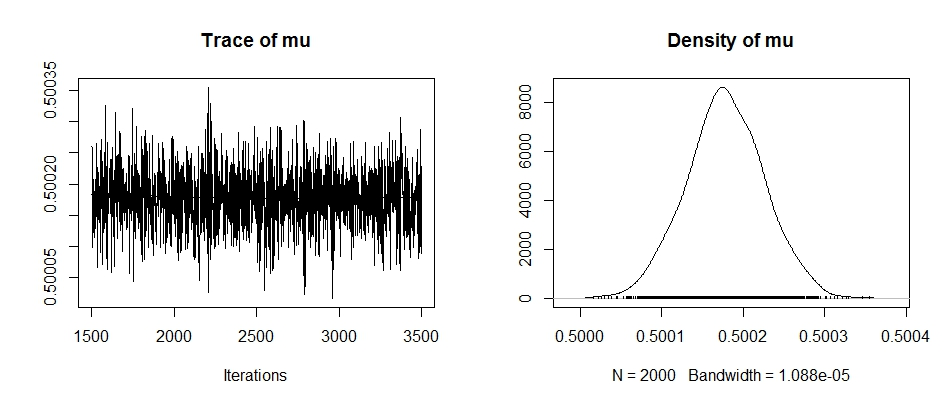
\includegraphics[width=0.7\linewidth]{Week3_MCMCRplot}
	%\caption{}
	\label{fig:week3mcmcrplot}
\end{figure}

We can also print out the summary of $\verb|mod_sim|$, which summarizes the iteration of the chain, and the statistics of the parameter variable $\mu$

\begin{lstlisting}
> summary(mod_sim)

Iterations = 1501:3500
Thinning interval = 1 
Number of chains = 1 
Sample size per chain = 2000 

1. Empirical mean and standard deviation for each variable,
plus standard error of the mean:

Mean             SD       Naive SE Time-series SE 
5.002e-01      4.782e-05      1.069e-06      1.361e-06 

2. Quantiles for each variable:

2.5%    25%    50%    75%  97.5% 
0.5001 0.5001 0.5002 0.5002 0.5003 
\end{lstlisting}

To access the vector $\mu$ and find the equal-tailed credible interval, we do
\begin{lstlisting}
> mu_post <- as.vector(mod_sim[[1]])
>
> # To obtain the equal-tailed credible interval of "mu"
> quantile(mu_post, c(0.025, 0.975))
     2.5%     97.5% 
0.5000836 0.5002727
\end{lstlisting}

The result shows that the \textbf{equal-tailed credible interval} of $\mu$ after the MCMC simulation is [0.5000836, 0.5002727].\\

To get the highest probability density credible interval, we do
\begin{lstlisting}
> HPDinterval(mod_sim)
[[1]]
lower     upper
mu 0.5000854 0.5002736
attr(,"Probability")
[1] 0.95
\end{lstlisting}

The \textbf{highest probability density credible interval} of $\mu$ is [0.5000854, 0.5002736], which does not differ too much from the equal-tailed credible interval.

To get the marginal distribution of $\bar{Y}$ under $\mu$
$$ \int f(\bar{y}~|~\mu, H_2)\pi(\mu~|~H_2)\, d\mu, $$
we implement the Monte Carlo simulation again. 

\begin{lstlisting}
> y_post = rnorm(length(mu_post), mean = mu_post, sd = 0.5 ^ 2 / 104490000)
>
> # Highest probability density credible interval of y_bar
> HPDinterval(as.mcmc(y_post))
         lower     upper
var1 0.5000865 0.5002747
attr(,"Probability")
[1] 0.95
\end{lstlisting}

The credible interval of $\bar{Y}$ is about [0.5000865, 0.5002747], which also implies that $\bar{Y}$ differs from 0.5. This means using the robust prior Cauchy distribution for $\mu$, the Bayesian approach also favors the alternative hypothesis.

\end{document}


